\section{Definitions and Equations}
\begin{figure}
    \centering
    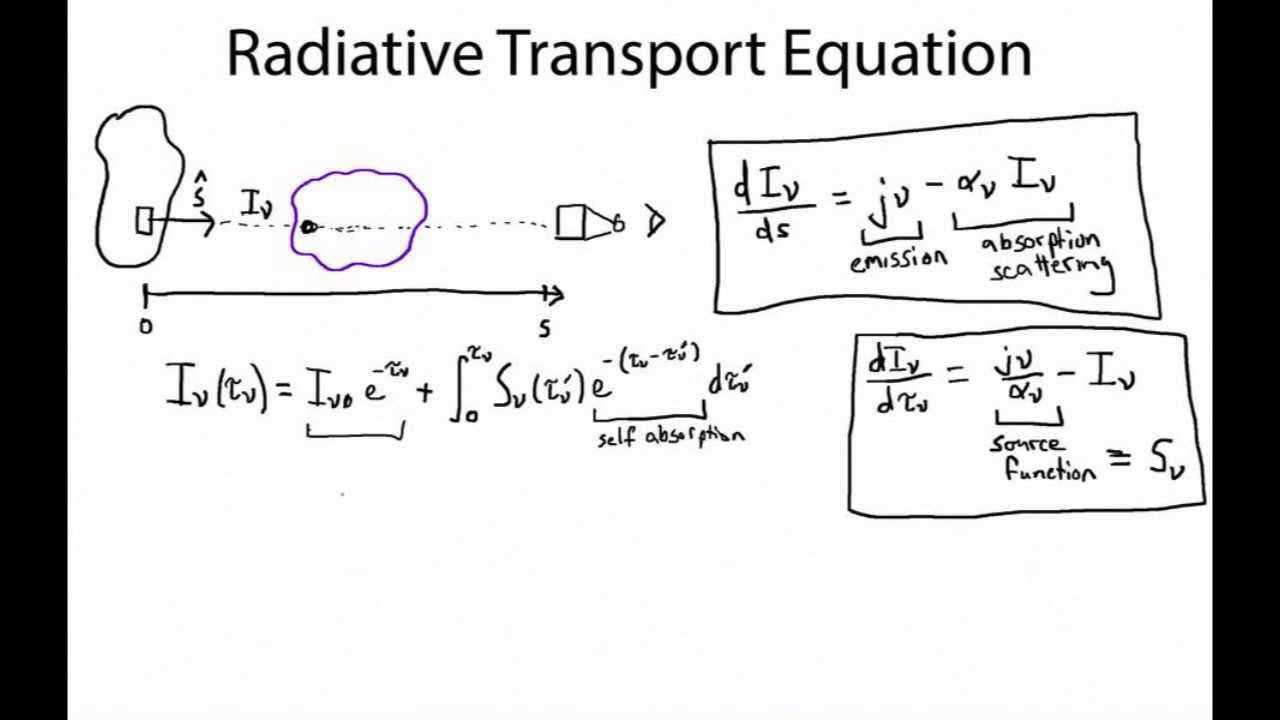
\includegraphics[scale=0.35]{maxresdefault.jpg}
    \caption{Accurate Figure}
    \label{fig:my_label}
\end{figure}
\begin{itemize}
    \item{Intensity: brightness of a ray as it passes through a medium. The units of intensity are [ergs / s / cm$^{2}$ / Hz/ str].
    \begin{align}
    I = \frac{dE}{dA\;d\Omega\;dt\;d\nu}
    \end{align}
    }
    \item{Radiative Transfer: How the intensity from some source interacts with material along the line of sight. This can involve absorption, emission, and scattering.
    \begin{align}
    I_{\nu} = I_{0} e^{-\tau_{\nu}} + S_{\nu} (1 - e^{-\tau_{\nu}})
    \end{align}
    }
    \item{Optical Depth: dimensionless quantity, tells how much the material has absorbed along line of sight.
    \begin{align}
        d\tau_{\nu} = \alpha_{\nu} ds = \kappa_{\nu} \rho ds
    \end{align}
    Where, $\kappa_{\nu}$ and $\rho$ are the opacity and density respectively.
    }
    \item{Source Function: The ratio of the emissivity to absorption coefficient. These are intrinsic to the material. In the limit of local thermodynamic equilibrium, the source function becomes a blackbody.
    \begin{align}
    S_{\nu} = j_{\nu} / \alpha_{\nu} = \frac{n_{u} A_{u \ell}}{n_{\ell} B_{\ell u} - n_{u} B_{u \ell}}
    \end{align}
    }
    \item{Blackbody Function: Intensity at a specific frequency due to the temperature of the material.
    \begin{align}
        B_{\nu} = \frac{2h\nu^{3} / c^{2}}{e^{h\nu/kT} - 1}
    \end{align}
    }
    \item{Thermal emission: occurs when collisional processes dominate over radiative processes. Stats given by Maxwell-Boltzmann statistics so that S$_\nu$ \rightangle B$_\nu$. Becomes blackbody when optically thicc
    \begin{align}
        \frac{n_{u}}{n_{\ell}} = \frac{g_u}{g_\ell}e^{-h\nu/kT}
    \end{align}
    Where $n$ describes the level populations, and $g$ are the degeneracies in each energy level.
    }
    \item{Rayleigh-Jeans Approximation: The Planck function can be approximated using this equation at low frequencies ($h\nu<<kT$).
    \begin{align}
    I_{\nu}^{\rm RJ} = \frac{2\nu^{2}}{c^{2}} kT
    \end{align}
    }
    \item{Wien's Approximation: The Planck function can be approximated using this equation at high frequencies ($h\nu>>kT$).
    \begin{align}
    I_{\nu}^{W} = \frac{2h\nu^{3}}{c^{2}}e^{-h\nu/kT}
    \end{align}
    }
    \item{Specific Energy Density:
    \begin{align}
    U_{\nu} = \frac{I_{\nu}}{c}
    \end{align}
    }
    \item{Angular Averaged Intensity:
    \begin{align}
    J_{\nu} = \frac{1}{4\pi} \int I_{\nu} d\Omega
    \end{align}
    }
\end{itemize}

\section{Kirchoff's Laws}
\begin{itemize}
    \item{
    \begin{enumerate}
        \item{No background emission ($I_{0} = 0$):
        \begin{align}
        I_{\nu} = S_{\nu} (1 - e^{-\tau_{\nu}})
        \end{align}
        \begin{enumerate}
            \item{Optically thin ($\tau << 1$). $S_{\nu}$ goes to $B_{\nu}$ in thermal equilibrium.
            \begin{align}
            I_{\nu} = S_{\nu}\tau_{\nu}
            \end{align}
            }
            \item{Optically thick ($\tau >> 1$). $I_{\nu} = S_{\nu} = B_{\nu}$ in local thermodynamic equilibrium.}
        \end{enumerate}
        }
        \item{Background emission
        \begin{enumerate}
            \item{Optically thin:
            \begin{itemize}
                \item{If $I_{0} > S_{\nu}$, we see an absorption line:
                \begin{align}
                    I_{\nu} = I_{0} - \tau_{\nu} (I_{0} - S_{nu})
                \end{align}
                }
                \item{If $S_{\nu} > I_{0}$, we see an emission line:
                \begin{align}
                    I_{\nu} = I_{0} - \tau_{\nu} (S_{nu} - I_{0})
                \end{align}
                }
            \end{itemize}
            }
            \item{Optically thick:
            \begin{align}
                I_{\nu} = S_{\nu}
            \end{align}
            }
        \end{enumerate}
        }
    \end{enumerate}
    }
\end{itemize}

\section{Scattering}

    \begin{align}
        \frac{dI_{\nu}}{ds} = -(\alpha_{\nu} - \sigma_{\nu,s}) (I_{\nu} - B_{\nu})
    \end{align}
    Where, $\sigma_{\nu,s}$ is the absorption cross-section.
    \begin{align}
        \ell_{*} \simeq \sqrt{N}\ell
    \end{align}
    Where $\ell$ is the mean free path, $N$ is the number of scattering events, and $\ell_{*}$ is the displacement from the center.
    \begin{align}
        \ell = \frac{1}{n\sigma}
    \end{align}
    The number of scattering events can be approximated as
    \begin{align}
        N \sim 1 - e^{-\tau_{\nu}}
    \end{align}

